% !TeX root = ../Bachelorarbeit.tex
\chapter{Einleitung}
\label{cha:Einleitung}

\section{Hinführung}
\label{sec:hinfuhrung}\index{Hinführung}
Im Jahr 2017 alleine wurden mehr als 1,8 Milliarden browser-fähige Endgeräte weltweit verkauft.\cite{statista_absatz} Der technologische Fortschritt in Hardware und Software geben dieser großen Masse an Zugängen zum Internet eine riesige Vielfalt an unterschiedlichsten Applikationen, die nahezu überall auf der Welt benutzbar sind. Einen großen Anteil machen dabei Spiele aus. Dabei haben auch Spiele auf mobilen Plattformen, wie Smartphones, immer mehr Grafikdetails und Leistungsanforderungen. Aber auch der Trend der Spieleklassiker ist immer noch belebt und beliebt: Klassische Spieleplattformen, wie der Commodore 64 und die Atari-Spielekonsole bekommen Neuauflagen\footnote{Auflistung von Neuauflagen bekannter Konsolen:\\ \url{http://www.computerbild.de/fotos/cbs-News-PC
-Bilder-Die-coolsten-Kultkonsolen-Remakes-18443703.html}} und auch klassische Spiele werden immer wieder für diverse Plattformen neu aufgelegt. Sie gehen dem Drang nach mehr Grafikdetails und Leistungshunger aus dem Weg gehen und sollen durch Charme mit Pixeln und Nostalgie punkten.\\
Spiele wurden für die Vorreiter des Konsolen- und Heimcomputermarktes, den Commodore 64 und die Atari, in Massen entwickelt.\footnote{Es wurden etwa 17.000 kommerzielle Titel entwickelt.\cite{commodore64}}
Die beliebtesten Spiele waren dabei unter anderem die Folgenden:\footnote{Auszug aus Liste nach \url{https://www.c64-wiki.de/wiki/C64-Wiki:TOP-Liste_des_C64-Wiki}}
\begin{itemize}
	\item Pirates
	\item Maniac Mansion
	\item Turrican \rom{2}
	\item Archon
	\item The Great Giana Sisters
	\item ...
\end{itemize}
Mit dabei ist auch das Spiel, um das sich diese Arbeit dreht: \emph{Archon}.\\
\index{Archon!Cover}
\begin{figure}[htp]
\centering
\captionsetup{justification=centering}
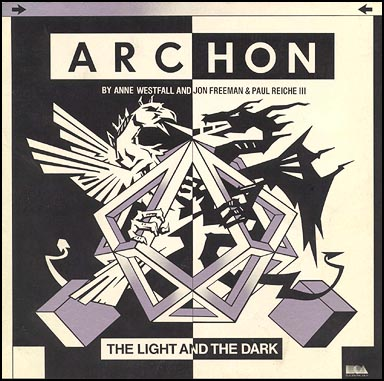
\includegraphics[width=0.50\textwidth]{Archon.jpg}
\caption[Archon - Cover]{Archon - Cover\footnotemark}
\label{fig:Archon_Cover}
\end{figure}
\footnotetext{\Quelle{C64-Wiki, \url{https://www.c64-wiki.com/wiki/Archon}}}\\
Archon genoss für Atari und Commodore 64 großen Erfolg, ähnlich vieler anderer Spiele für die Konsolen der 80er. Auch hat Archon schon einige Neuauflagen und Nachfolger bekommen.\footnote{Eine Neuauflage ist Archon Classic: \url{https://store.steampowered.com/app/65400/Archon_Classic/}}
Die meisten davon wurden für den Computer entwickelt. Der Computer ist jedoch nicht die einzige Plattform für Spiele.
Plattformen für Spiele gibt es genügend für jeden Geschmack: Ob Konsole -- die \ggf tragbar ist --, Computer, Smartphone oder Webbrowser.
Die klaren Vorteile des Web als Plattform, auch für Spiele, sind dabei die Offenheit, der einfache Zugang und die immer weiter steigende Unterstützung neuer, standardisierter Technologien.\\
So sind heutzutage hardwarebeschleunigte\footnotemark{} 3D-Visualisierung und Echtzeitkommunikation im Webbrowser Stand der Technik.
In dieser Arbeit soll daher die Verschmelzung von State of the Art Webtechnologien mit einem Spieleklassiker erfolgen.\\\footnotetext{Hardwarebeschleunigung entlastet den Prozessor durch Auslagerung an spezialisierte Hardware für bestimmte Aufgaben.}

\section{Aktueller Forschungsstand}
\label{sec:aktueller_forschungsstand}\index{Forschungsstand}
\noindent Dieses Kapitel behandelt den Einstieg in aktuelle Themen der Spieleentwicklung und des Internets. Zunächst wird dabei auf aktuell stark behandelte Themen des World Wide Web Consortium (W3C) -- dem Konsortium zur Standardisierung des Web--, eingegangen. Dabei wird das Thema Grafik im Web noch einmal gesondert eingeführt. Abschließend wird auf aktuelle Probleme, Herausforderungen und Eigenschaften der heutigen Spieleindustrie eingegangen.

\subsubsection{aktuelle Themen des W3C}
Das W3C hat im Moment neun Kernthemen im Rahmen "Web Design and Applications".\\
Mit MathML soll ein Standard für die Anzeige von mathematischen Ausdrücken geschaffen werden. Weiterhin wird in den Themen "Privacy", "Accessibility", "Internationalization" und "Mobile Web" stark geforscht und an Standards gearbeitet um möglichst jedem Menschen der Welt, mit jedem internetfähigen Gerät, den vollen und sicheren Zugang zum Internet zu ermöglichen. Die in dieser Auflistung noch fehlenden Themen sind "Audio \& Video", "JavaScript Web APIs"\footnote{Application Programming Interface (API) -- Eine Schnittstelle zum programmatischen Zugriff auf eine Anwendung} sowie "Graphics".\footnote{Die Themen sind dem W3C direkt entnommen: \url{https://www.w3.org/standards/webdesign/}}
Das Thema "Audio \& Video" behandelt vor allem die Standardisierung von Formaten von Audio- \& Videoinhalten. "JavaScript Web APIs" dienen der Entwicklung von umfangreicheren clientseitigen Web-Anwendungen.

\noindent Das Thema "Graphics" behandelt nicht nur Formate zu Darstellung, sondern auch Schnittstellen zur dynamischen Erzeugung und Veränderung, von Grafiken. Die Schnittstellen "Scalable Vector Graphics" (SVG) und die "Canvas API" sind in diesem Zusammenhand zu nennen. Sie werden beide inzwischen von den meisten, modernen Browsern unterstützt. Beide Schnittstellen erlauben die dynamische Erzeugung und Manipulation von zweidimensionalen (2D) Grafiken. Für dreidimensionale (3D) Grafiken ist allerdings noch kein Standard des W3C ausgearbeitet worden. Es gibt allerdings den "WebGL" Standard, welcher von der "Khronos Gruppe" ausgearbeitet wurde.\footnote{Für weitere Informationen zur Khronos Gruppe: \url{https://www.khronos.org/webgl/}} Der Standard erlaubt es der "Canvas API" einen neuen Kontext zu geben und damit 3D-Grafiken zu erzeugen. Die meisten, modernen Browserhersteller sind Teil der Arbeitsgruppe zur Erstellung des Standards.

\subsubsection{aktuelle Themen der Spieleindustrie}
Spielen sind heutzutage kaum noch Grenzen gesetzt. Mit "Virtual Reality" (VR), teilweise Millionen von Spielern -- auf der ganzen Welt verteilt--, oder auch höchsten Anforderungen an Rechen- und Kommunikationsleistung bringen Entwickler auch aktuelle Hardware teils an ihre Grenzen. Dabei entstehen, dank der teils riesigen Budgets\footnote{Siehe \url{https://en.wikipedia.org/wiki/List_of_most_expensive_video_games_to_develop}}, unglaubliche, digitale Welten.\\
Weiterhin wird immer größerer Fortschritt im Bereich der künstlichen Intelligenz gemacht, die auch für die Spieleindustrie eine große Rolle spielt.\footnote{Siehe dazu: \url{https://openai.com/}}
\section{Motivation / Problemstellung}
\label{sec:motivation}\index{Motivation}
Bisher sind oftmals nur Demonstrationen, kurze Starter-Kits \bzw Einstiegspunkte einzelner Web-Technologien und Frameworks im Web zu finden. Anhand dieser Arbeit sollen die Möglichkeiten des Webs in ihrer Gesamtheit dargestellt werden und die Realisierbarkeit von 3D-Spielen für Webbrowser aufgezeigt werden. Weiterhin kann das Spiel als Beispiel für typische Problemstellungen eines Entwicklers für Browserspiele dienen.\\
Versionen, Ableger und Kopien des Spieleklassikers Archon gibt es zahlreich. Meist sind diese jedoch auf ein System beschränkt, oder tatsächlich nur mit einem Emulator\footnote{Emulator -- Ein Emulator simuliert ein anderes System (\zB Spielekonsolen werden auf einem Computer emuliert)} ausführbar. Das Web leistet an dieser Stelle die perfekte Abhilfe: Es gibt unzählige Geräte, die heutzutage einen Webbrowser installiert haben, somit kann jeder Zugriff auf diesen Ableger haben, der ein webfähiges Gerät besitzt.
\clearpage
\section{Zentrale Begriffe}
\label{sec:zentrale_begriffe}\index{Zentrale Begriffe}
\subsection{Was versteht man unter Webtechnologien?}
Webtechnologien betiteln meist die Sammlung aller technischen Aspekte zum Erstellen, Warten und Entwickeln einer Webanwendung.\\
Webanwendungen selbst bestehen immer aus einem Client-Server-Modell. Dabei stellt, auf Anfrage eines Clients, der Server passende Inhalte für den Client bereit. Der Client wird dabei meist von einem Webbrowser repräsentiert, der die Anfragen an Webserver sendet und Antworten empfängt. Der Webbrowser ist dabei für die anschließende korrekte Interpretierung der Antworten zuständig.
Typische Bestandteile des Clients und ihre Bedeutungen sind: 
\begin{itemize}
	\item Hypertext Markup Language (HTML) zur Beschreibung von Inhalt und seiner Struktur
	\item Cascading Style Sheets (CSS) zur Beschreibung des Aussehens des Inhalts
	\item JavaScript zur Dynamisierung des Clients und der gesendeten Inhalte
\end{itemize}
Ein Webserver ist eine Anwendung, die auf Anfragen von Webprotokollen, wie dem Hypertext Transer Protocol (HTTP), mit Inhalten und Daten antworten kann. Ein Webserver kann dabei noch weitere Eigenschaften haben, wie Fehlerverarbeitung, Verschlüsselung der Kommunikation oder Verwaltung einer Datenbank für Anwendungsdaten.
\subsection{Was versteht man unter 3D-Technologien?}
Da ein Bildschirm, beispielweise eines Computers, nur zweidimensional ist, muss durch andere Methodiken der Effekt einer dritten Dimension geschaffen werden. Wie dieser Prozess im Allgemein funktioniert wird folgend erläutert.\\Objekte im 3D-Raum werden über ihre Eckpunkte aufgespannt und im Code somit in einem 3D-Raum mit normalem 3-Achsen-Koordinatensystem dargestellt. Anschließend folgt der Prozess des Renderns, bei dem zunächst aus den einzelnen Punkten der Objekte die Formen errechnet werden, indem die Eckpunkte zu Flächen verbunden werden. Anschließend erfolgt eine Ausrichtung aller Flächenpunkte am Pixel-Raster des Bildschirms, sodass eine 3D-Projektion der 2D Pixel entsteht. Der nächste Schritt, Fragment-Bearbeitung, behandelt die Einfärbung der, im vorherigen Schritt gebildeten, "Fragmente" anhand von Licht und verwendeten Texturen. Der finale Schritt des Renderns wandelt die 3D-Projektion in ein 2D-Pixel-Bild, dass dann auf dem Bildschirm angezeigt wird. Außerdem werden im letzten Schritt Prüfungen für die Sichtbarkeit von Objekten unternommen, sodass nicht sichtbare Objekte, oder Teile von ihnen, auch nicht weiter verarbeitet werden.

\section{Ziel dieser Arbeit}
\label{sec:ziel_dieser_arbeit}\index{Ziel}
Der Schwerpunkt dieser Arbeit befasst sich mit der Umsetzung des bekannten Spieleklassikers Archon mit Web- und 3D-Technologien.
Ziel dieser Arbeit ist es eine Webapplikation zu erstellen, die den Spieleklassiker Archon in einem 3D-Stil widerspiegelt.
Die Webapplikation soll dabei folgende generelle Anforderungen erfüllen, die im Laufe dieser Arbeit näher spezifiziert werden:
\begin{itemize}
	\item Die Applikation muss mittels Webtechnologien implementiert werden
	\item Das Spiel muss in einem 3D-Stil angezeigt werden
	\item Das Spiel muss als solches wiedererkennbar sein
\end{itemize}
\section{Aufbau}
\label{sec:aufbau}\index{Aufbau}

Im ersten Teil dieser Arbeit sollen die Anforderungen an eine Neuauflage von "Archon" erfasst werden und eine Beschreibung der Features und Spielmechaniken zur Umsetzung erstellt werden.
Darauffolgend werden die Anforderungen der technologischen Seite herausgearbeitet, sodass eine Liste an Funktionalitäten entsteht, die von den 3D- und Webtechnologien erfüllt werden muss.
Anschließend wird der Aufbau der Entwicklungsumgebung, sowie benutzte Hilftmittel und getroffene Vereinfachungen beschrieben.
Alle Anforderungen werden dann in eine Beschreibung zur Umsetzung und in eine entsprechende Architektur ausgearbeitet.
Die Implementierung wird in Ausschnitten gezeigt, die die einzelnen Schritte und die Vorgehensweise bei der Umsetzung von Architektur und Programmierung aufzeigen sollen.
Den Abschluss bildet eine Überprüfung auf die Erfüllung der Anforderungen mit kurzem Einblick auf den abschließenden Stand und eine Reflexion des Ergebnisses mit Ausblick auf Folgearbeiten an der Webapplikation.